\documentclass[a4paper, 12pt, oneside, table]{article}
\usepackage[square, numbers, comma, sort&compress]{natbib}  % Use the "Natbib" style for the references in the Bibliography
\usepackage{verbatim} 
\usepackage[english]{babel}
\usepackage[utf8]{inputenc}
\usepackage{graphicx}
\usepackage{multirow}
\usepackage{amsmath}
\usepackage{amssymb}


%\usepackage{cite}
\usepackage{booktabs}
\usepackage{listings}
\usepackage{epstopdf}
\usepackage{helvet} 
\renewcommand{\familydefault}{\sfdefault}
\usepackage{setspace}
\singlespacing % interlinea singola
\linespread{0.97}
\usepackage{color}
\usepackage[margin=2.5cm]{geometry}
\setlength{\parindent}{0pt}
% pacchetti aggiunti
\usepackage{comment}
\usepackage[export]{adjustbox}
\usepackage{subfigure}
%\usepackage{subcaption}
\usepackage{algorithm}
\usepackage{algorithmic}
\usepackage{amsfonts}
\usepackage{tabularx}
\usepackage{ltablex}
\usepackage{caption}
\usepackage{titling}
\usepackage{spreadtab}
\renewcommand\maketitlehooka{\null\mbox{}\vfill}
\renewcommand\maketitlehookd{\vfill\null}

\usepackage{comment}

\usepackage{mathtools}
\DeclarePairedDelimiter{\floor}{\lfloor}{\rfloor}

\usepackage{enumerate}
\usepackage{enumitem}
\usepackage[dvipsnames]{xcolor}
\newcommand*{\lorenzo}[1]{\textcolor{BurntOrange}{#1}}
\newcommand{\yasmin}[1]{\textcolor{Red}{#1}}
\newcommand{\giovanni}[1]{\textcolor{Blue}{#1}}


\title{RASD}
\author{Yasmin Awad, Lorenzo Carpaneto, Giovanni Dispoto}
\date{November 2020}

\begin{document}

\begin{titlepage}
%\vspace*{\fill}
\begin{figure}[h!]
	\centering
	
\includegraphics[scale=0.5]{img/logopoli.png}
\end{figure}
\vspace{0.7em}
\begin{center}
	\Large \textbf{DD}
\end{center}
%\begin{center}
%	\large Version 0.1
%\end{center}
%\begin{center}
%	\large Version Date
%\end{center}
%\vspace{0.4em}
\begin{center}
	\Large \textbf{CLup – Customers Line-up } 
\end{center}
\vspace{-0.6em}
\begin{center}
	\normalsize Yasmin Awad, Lorenzo Carpaneto, Giovanni Dispoto
	\begin{figure}[h!]
	\centering
	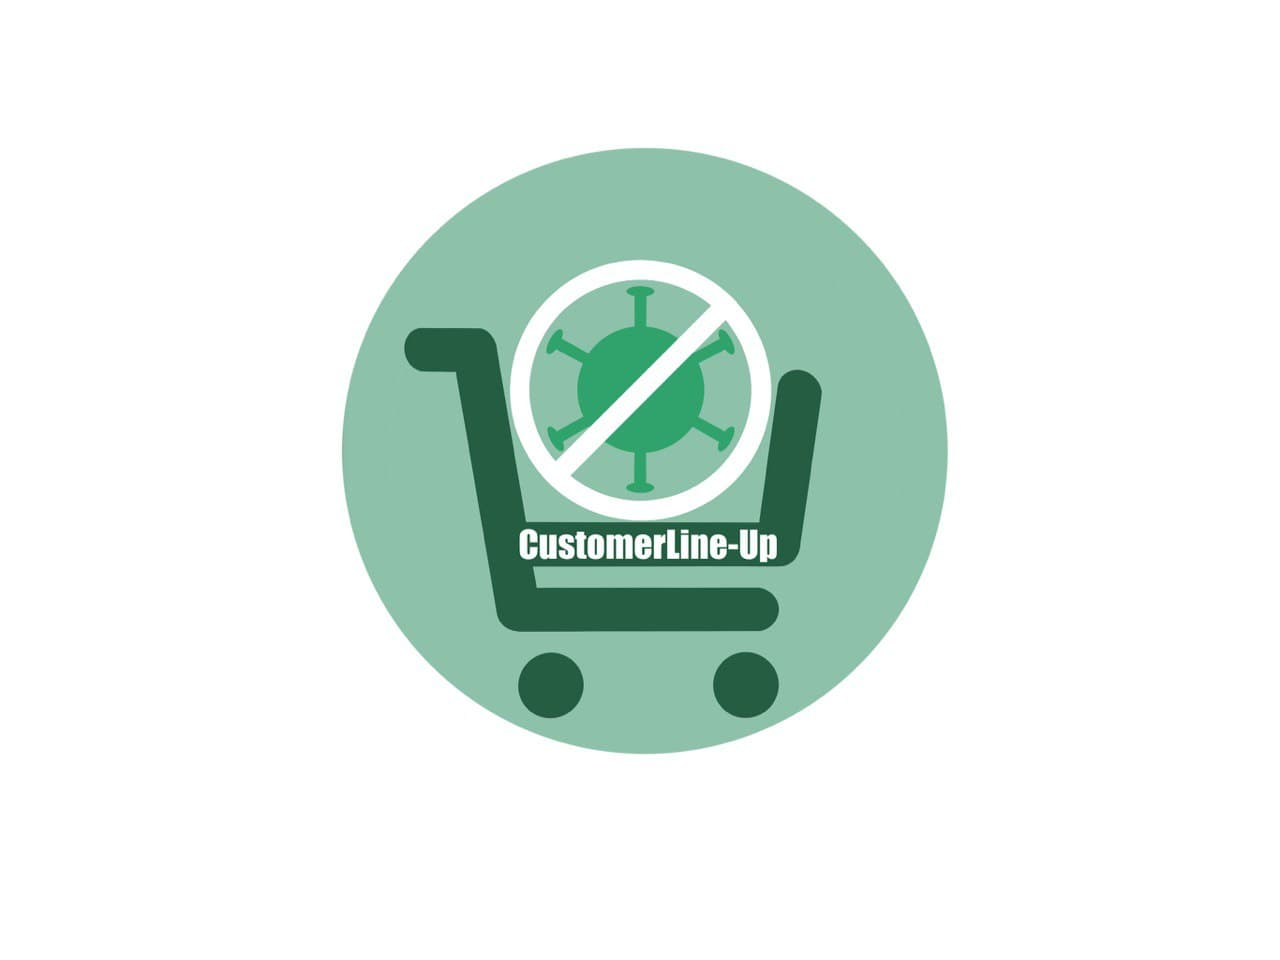
\includegraphics[scale=0.25]{img/logo.jpg}
\end{figure}
\end{center}
\vspace*{\fill}
\end{titlepage}

\normalsize


\newpage
\tableofcontents
\newpage

\section{Introduction}
\subsection{Purpose}
After showing a general description of the CL-up application within the RASD, this document focuses on analyzing the system's architecture and design, in order to satisfy the various requirements stated in the previous document. The purpose of the document is to provide a functional description of the main architectural components, showing their runtime behaviour and interactions and their interfaces. This document is mainly intended to be used by the developers and testers.

\subsection{Scope}
Customer Line-up (CL-up) is an application that aims to allow accesses to Stores in a safe way. The objective is to avoid as much as possible queue formation outside the Stores and limits the number of people inside it in an efficient way. To pursue this goal, the application allows Users to register either as a Managers or Customers, providing services to both of them. Managers can create their Stores within the app and allow other Managers to help them in the organization of the Store rules. Tools are provided to allow Customers to book Visits or Tickets to the Stores remotely, allowing a greater and more efficient way for maintaining social distancing. This is done by the use of a virtual queue managed by the System, in which Customers' Reservations are stored and managed. In order to organize the various entrances in the Stores, an identifier for each Consumer will be used, that is a QRCode.\\ %The application provides also a fall-back option (Paper Tickets) and suggestions for Customers.
\\
More information can be found in the Chapter 1 of the RASD.

\newpage
\section{Architectural Design}
\subsection{Overview: High-level components and their interaction}
In this chapter the architectural structure of the System will be described. In Figure \ref{high_level_overview_img} the high level overview of the System is shown. In the next sections we will describe in detail the various components and their interactions.

\begin{figure}[h!]
\centering
	\centering
  	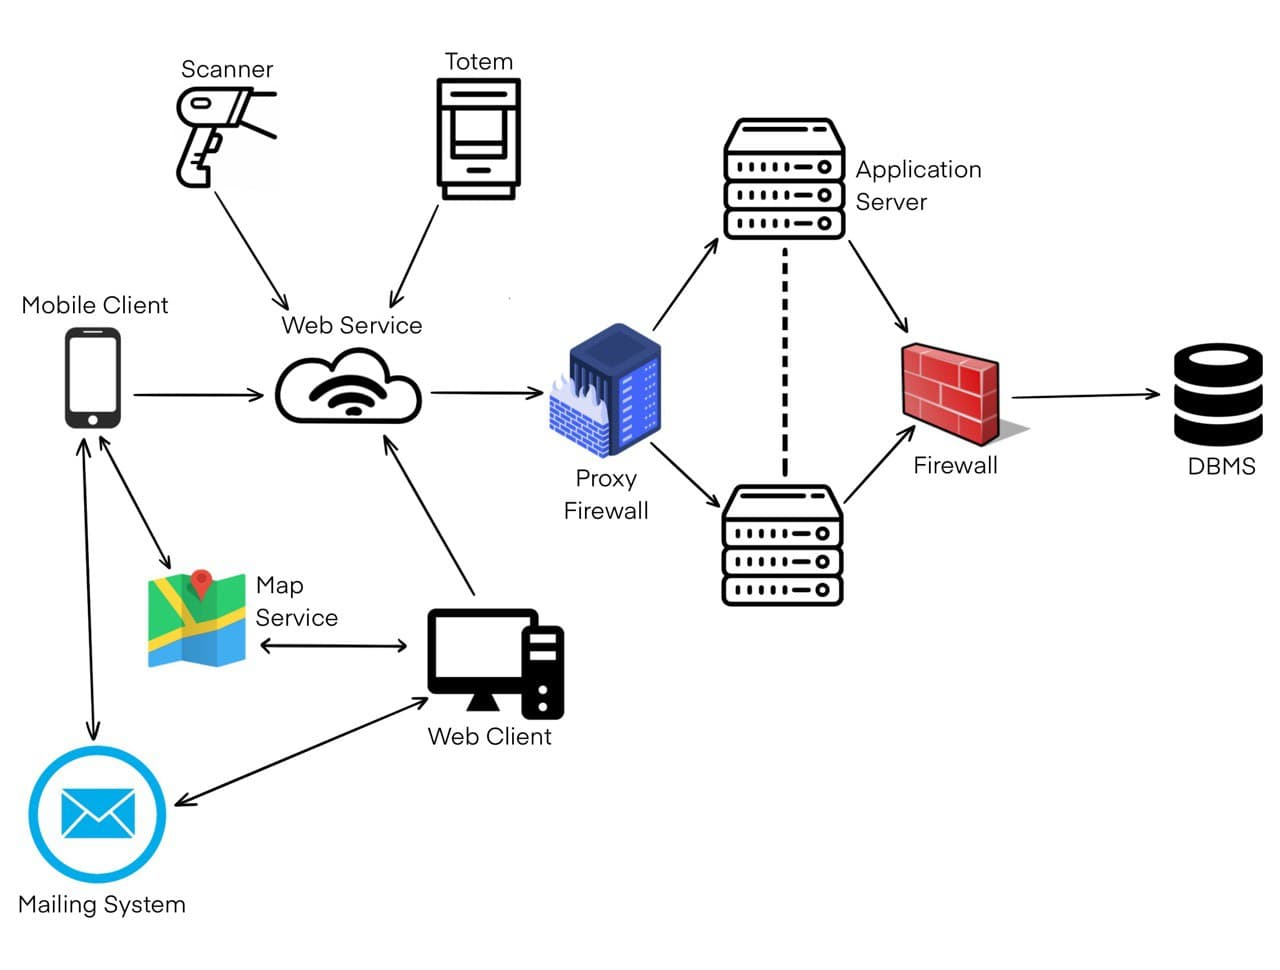
\includegraphics[height=0.4\textheight, scale=0.3, keepaspectratio]{img/high_level_overview.jpg}
	\caption{High-level overview of the System.}
 	\label{high_level_overview_img}
\end{figure}

\subsection{Component View}
To describe the internal modular structure of the components, we show how they are connected together in the UML component diagram in Figure \ref{comp_view_img} Components are wired together using an \textit{assembly connector} to connect the required interfave of one component with the provided interface of another component.

\begin{figure}[hbt]
\centering
	\centering
  	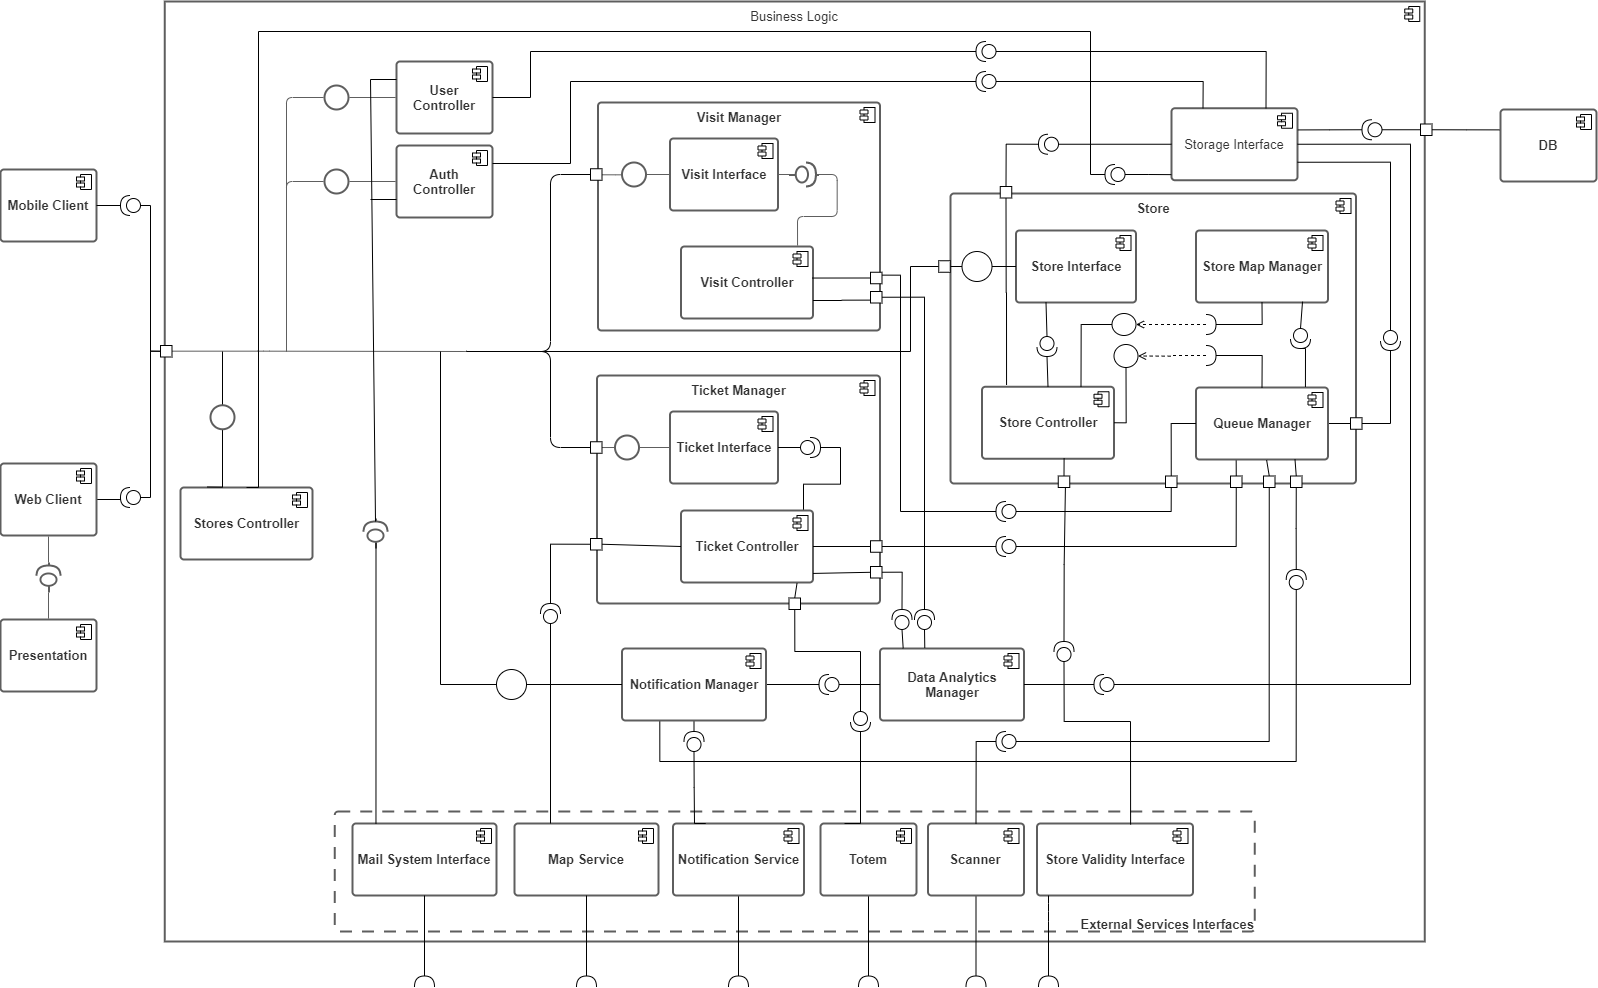
\includegraphics[height=0.4\textheight, scale=0.2, keepaspectratio]{img/component_view.png}
	\caption{Component diagram of the system.}
 	\label{comp_view_img}
\end{figure}

\begin{itemize}
    \item \label{cv:client}\textbf{Mobile Client} and \textbf{Web Client}: represents the two machines that accesses the entire System and it's functionalities. They both do not have important functions on their own, because we chose to implement them using a Thin Client approach.
    \item \textbf{Presentation}: it is used in order to display web pages of the application to a Web Client accessing through the browser. This layer only provides the structure of the user interface without accessing any data or application logic \lorenzo{forse metterei solo non accede all'application logic, perche' ai dati in qualche modo deve accederci per farli visualizzare su schermo (anche se puo' non sapere come siano stati estrapolati)}.
    \item \textbf{User Controller}: This component handles all the operations that affects the user data. It exposes method to change account credentials and stores them in the database.
    \item \textbf{Auth Controller}: This component handles all the operation for the authentication such as registration process and login process. It communicate with DBMS through Storage Interface in order to retrieve and insert user credentials. During the registration process or change password this component use Mailing System Interface
    \item \textbf{Data Analytics Manager}: is a component used in order to analyze Customers habits. In practice is a Recommender System that takes care of showing to a Customer the Stores most appealing to him and the best duration value to be included in a Reservation.
    \item \textbf{Notification Manger}: is a component used in order to provide Notifications to the Customer, such as  Virtual Tickets departures, appealing time slots of specific Stores and suggestions.
    \item \textbf{Ticket Manager}: is a subsystem component in charge of managing Ticket requests:
    \begin{itemize}
        \item \textbf{Ticket Interface}: it exposes to the Customer an Interface for compiling the requested Ticket attributes.
        \item \textbf{Ticket Controller}: it checks the validity of the inserted Ticket's attributes requested. Moreover it communicates with the Queue Manager in order to verify the possibility to accomplish the request.
    \end{itemize}
    \item \textbf{Visit Manager}:is a subsystem component in charge of managing Visit requests:
    \begin{itemize}
        \item \textbf{Visit Interface}: it exposes to the Customer an Interface for compiling the requested Visit attributes.
        \item \textbf{Visit Controller}: it checks the validity of the inserted Visit's attributes requested. Moreover it communicates with the Queue Manager in order to verify the possibility to accomplish the request.
    \end{itemize}
    \item \textbf{DB}: it represents the DBMS, which provide an interface to read and store data. User credentials, Stores information and queues reservations are stored  in the database.
    \item \textbf{Storage Interface}: it provide methods to access to database. This interface is needed in order to decouple all the components from the DBMS technology.
    \item \textbf{Store}: is a subsystem component in charge of managing Store and its Queue:
    \begin{itemize}
        \item \textbf{Store Interface}: it exposes to the Manager an Interface for creating and managing Stores.
        \item \textbf{Store Controller}: it ensures that a Manager intending to become Owner of a Store within the application has the necessary authorizations, checking the validity of the information by acquiring specific credentials. \yasmin{dovrei collegarlo a un external service di verifica??}
        \item \textbf{Queue Manager}: this component receives requests for Reservations for the Store, checks that they can be placed in the queue and eventually inserts them. It communicates with the Ticket Controller, the Visit Controller, the Scanner and the Totem. It also communicate with the DB in order to retrieve and modify all the necessary information.
        \item \label{comp:storeMapMan} \textbf{Store Map Manager}: this component receives requests from the Customers who has already booked a Visit. It has to populate the map with the path that the Customer should follow during their Visit inside the Store. It communicates with the Queue Manager to look at the specified departments by other people during the time-slot of the Visit specified.
    \end{itemize}
    \item \textbf{External Services Interfaces}: this set of components have as main objective to make API calls to the necessary third party services:
    \begin{itemize}
        \item \textbf{Mailing System Interface}: is an interface in charge of sending confirmation mails at the end of the registration process to the User. It also can send other type of notification mails.
        \item \textbf{Map Service}: this service is used in order to retrieve the necessary information about a Customer position. This information is used by the Data Analytics System and by the Ticket Controller \yasmin{???? ripensaci bene}
        \item \textbf{Totem \yasmin{Interface ?? forse meglio}}: since the Totem of a Store has the task of issuing Paper Tickets, it needs to communicate with the Ticket Controller in order to make requests and allow the effective issue of the requested Ticket. This component is in charge of the communication.
        \item \textbf{Scanner}: the Scanner application has the task of reading QR codes of Customers and Paper Tickets so that it can control the entries and exits from the Store. In order for it to carry out the correct checks, it needs to communicate with the Queue Manager to obtain the right information. This component is in charge of the communication.
        \item \textbf{Store Validity Interface}: Is used in order to check that the created store is a real store. To do this, it has to verify Special Credentials provided from the Owner.
        
        \item \textbf{Notification Service}: Is used from Notification manager in order to send push notifications to client application.
    \end{itemize}
    
\end{itemize}

\newpage
\section{User Interface Design}

\subsection{Mockup}
\begin{figure}[h!]
\centering
\begin{subfigure}
	\centering
  	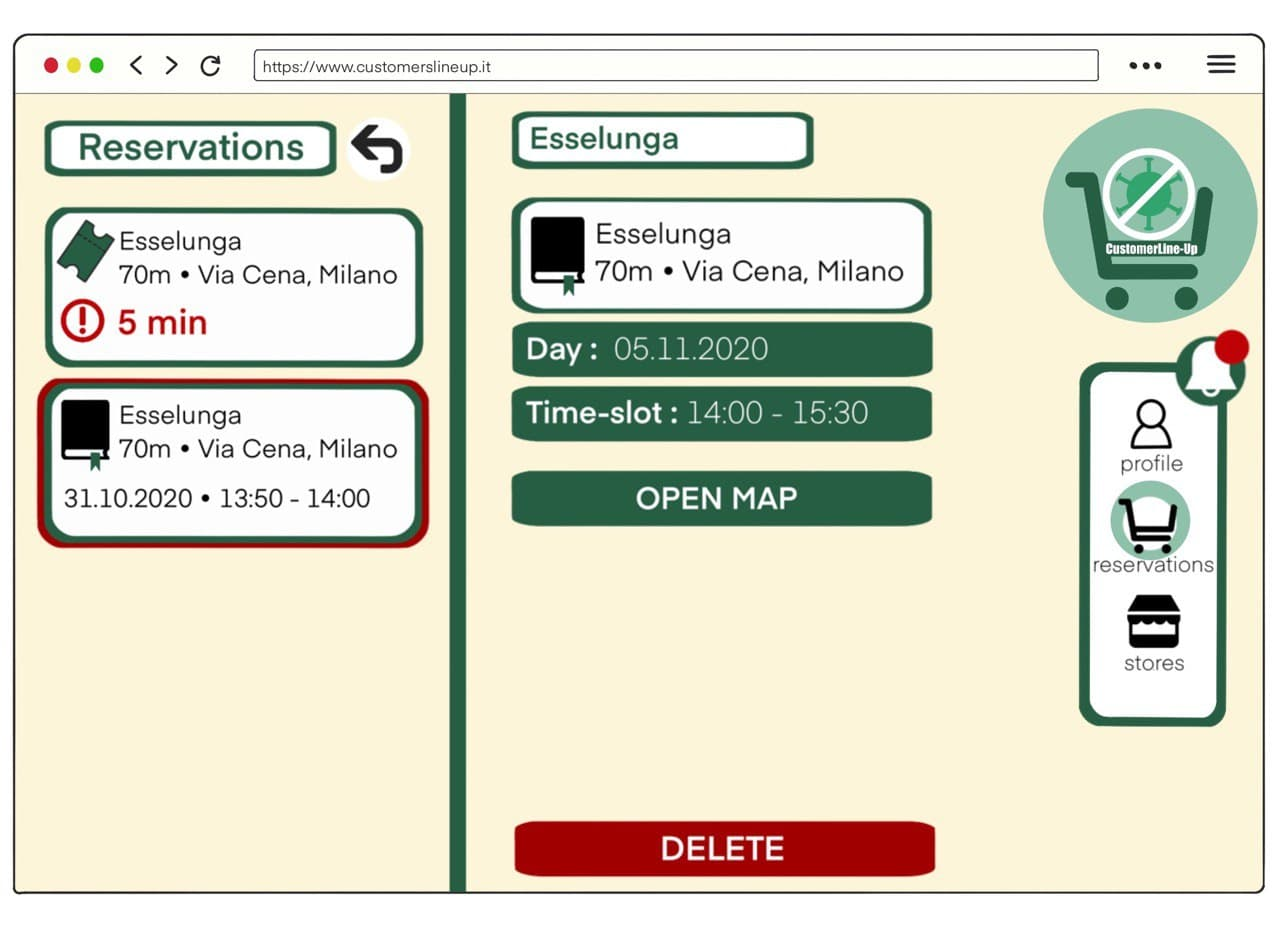
\includegraphics[height=0.4\textheight, scale=0.2, keepaspectratio]{img/customer_interface.jpg} 
 \end{subfigure}
 \begin{subfigure}
	\centering
  	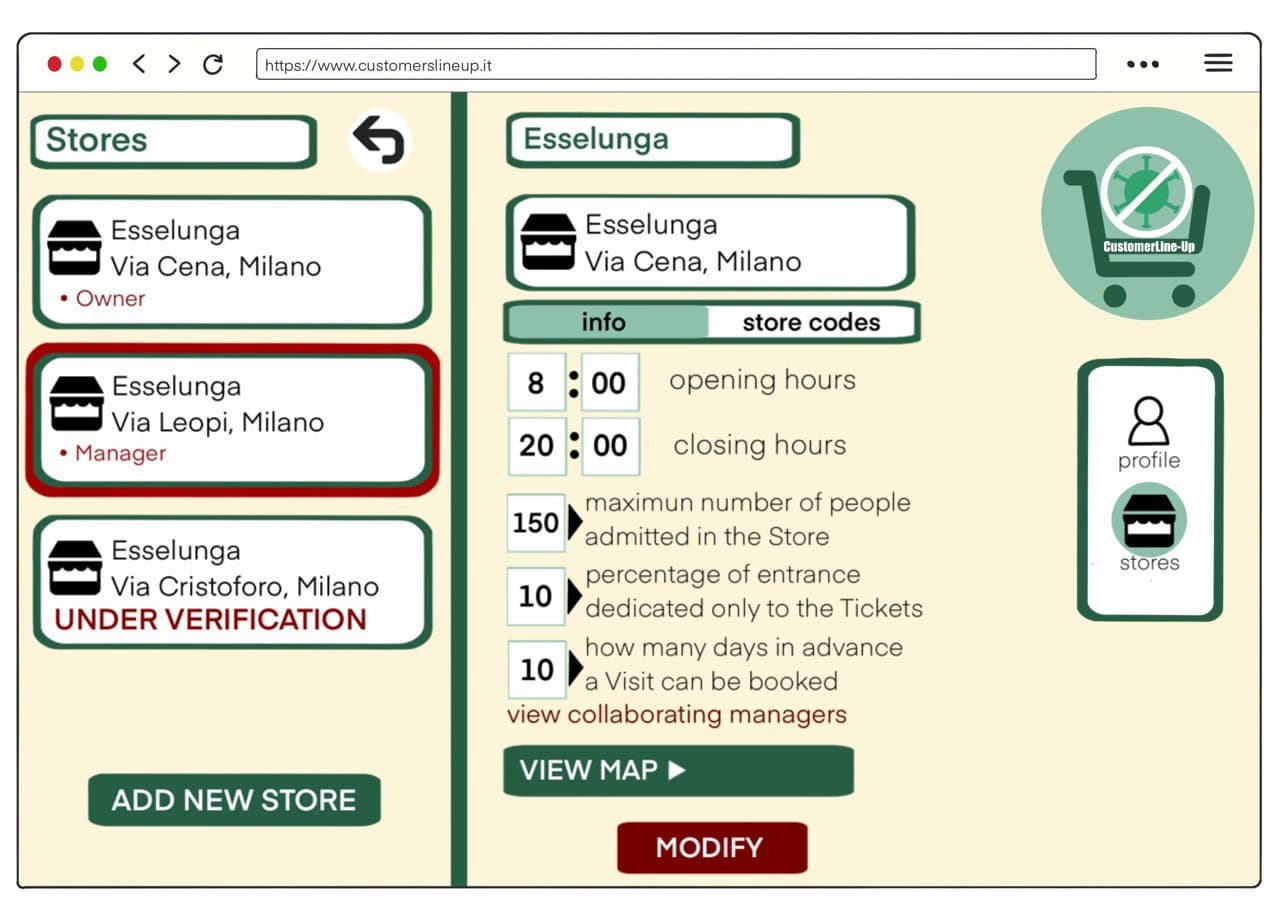
\includegraphics[height=0.4\textheight, scale=0.2, keepaspectratio]{img/manager_interface.jpg}
 \end{subfigure}
	\caption{Web page graphics.}
 	\label{web_graphics}
\end{figure}

\subsection{User Experience Diagram}
To better define the most important Users action within the application, we reported in Figure \ref{customer_experience} and in Figure \ref{manager_experience} two User Experience diagrams (UX), one for the Customer and one for the Manager. User Experience diagrams are diagrams that display the complete path a User takes when using a product, it refers to the functions and respective interfaces of the application.
\begin{figure}[h!]
\centering
	\centering
  	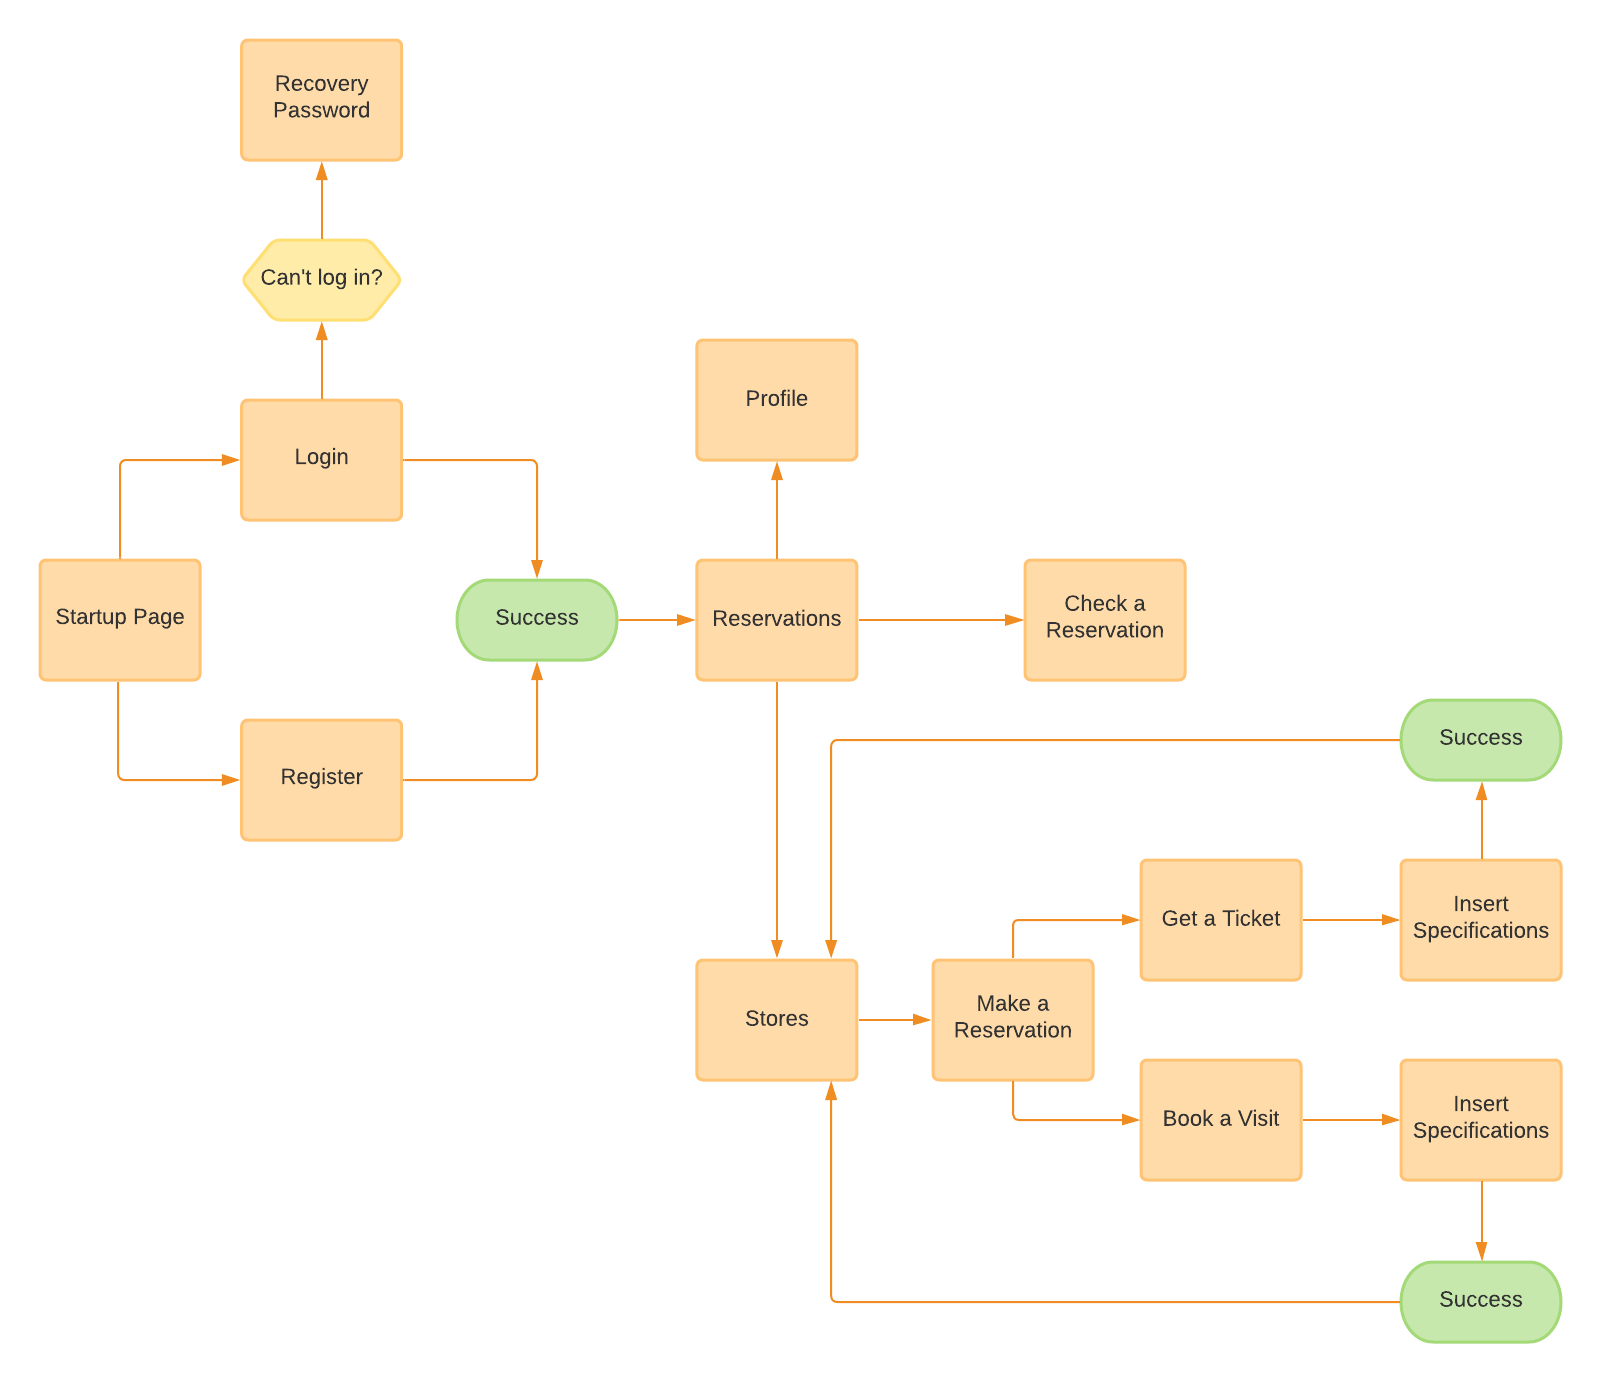
\includegraphics[height=0.5\textheight, scale=0.2, keepaspectratio]{img/customer_experience.png} 
  	\caption{UX flow of a Customer User.}
 	\label{customer_experience}
\end{figure}
\newpage
 \begin{figure}[h!]
	\centering
  	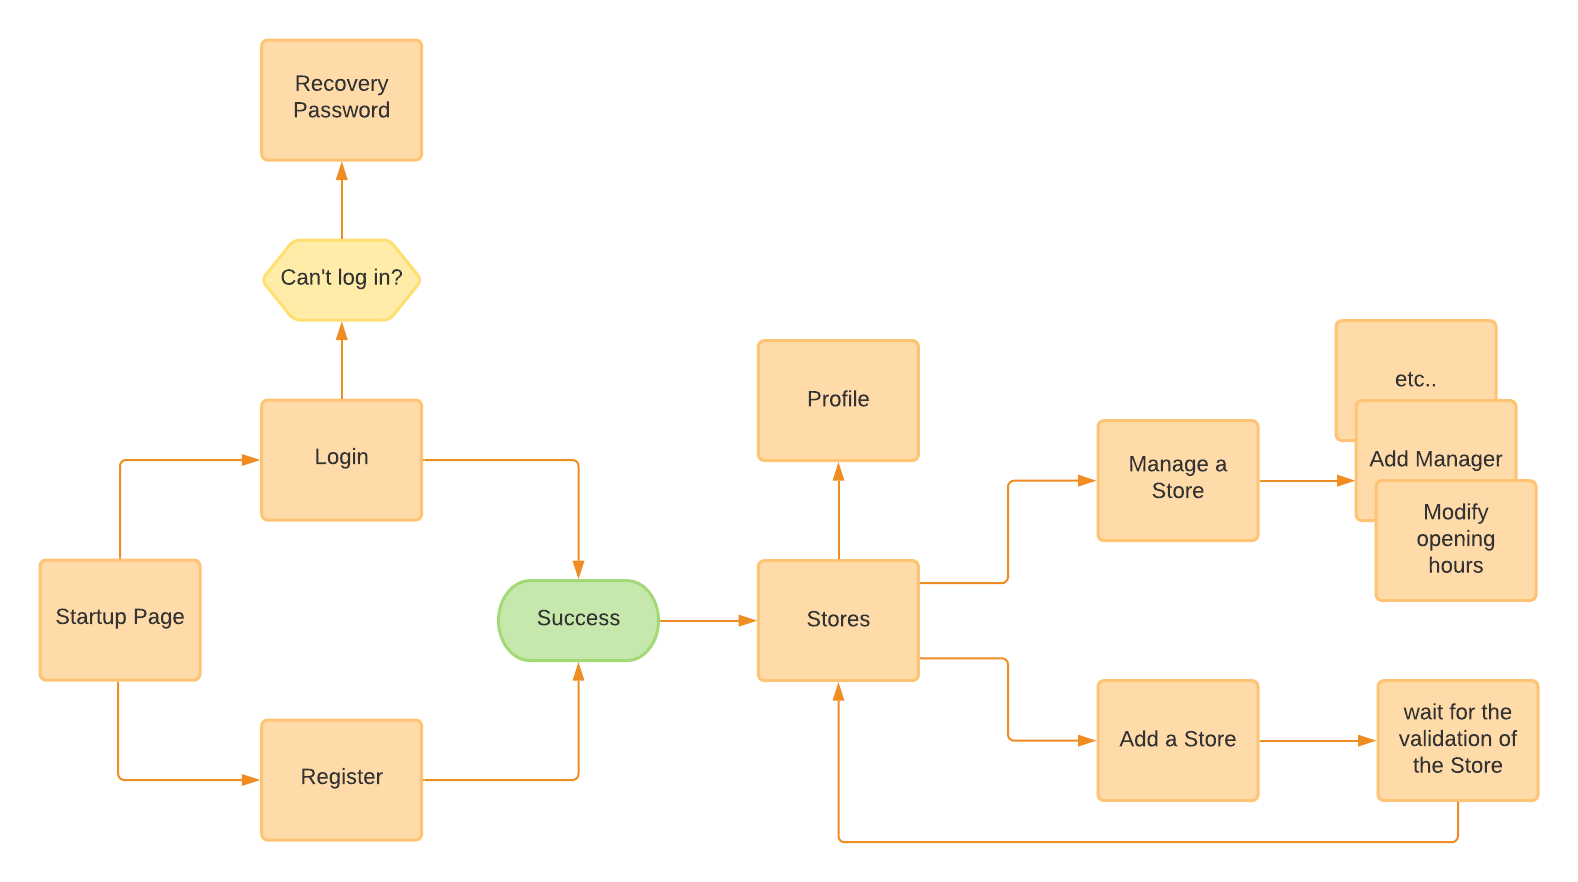
\includegraphics[height=0.35\textheight, scale=0.2, keepaspectratio]{img/manager_experience.png}
	\caption{UX flow of a Manager User.}
 	\label{manager_experience}
\end{figure}

\end{document}
